\documentclass[tikz,border=2pt,11pt]{standalone}
\usetikzlibrary{positioning}
\usetikzlibrary{arrows.meta}
\usetikzlibrary{patterns}
\usetikzlibrary{calc}
\usetikzlibrary{decorations.pathreplacing}
\usepackage{amsmath}
\usepackage{amssymb}
\usepackage{mathrsfs}
\usepackage{xcolor}
\usepackage{graphicx}
\usepackage{tikz}
\newcommand{\R}{\mathbb R}
\newcommand{\C}{\mathbb C}
\newcommand{\Z}{\mathbb Z}
\newcommand{\N}{\mathbb N}
\newcommand{\PP}{\mathbb P}
\newcommand{\EE}{\mathbb E}
\newcommand{\Peta}{\mathbb P^{\eta}}
\newcommand{\Eeta}{\mathbb E^{\eta}}
\newcommand{\Esp}{\mathbb E_{\mathrm{sp}}}
\newcommand{\eps}{\varepsilon}
\newcommand{\om}{\omega}
\newcommand{\ind}{\mathbf 1}
\newcommand{\dd}{\mathrm d}
\newcommand{\ii}{\mathrm i}
\DeclareMathOperator{\diam}{diam}
\DeclareMathOperator{\dist}{dist}
\DeclareMathOperator{\supp}{supp}
\DeclareMathOperator{\Area}{Area}
\DeclareMathOperator{\Var}{Var}
\DeclareMathOperator{\Rea}{Re}
\DeclareMathOperator{\Ima}{Im}
\begin{document}
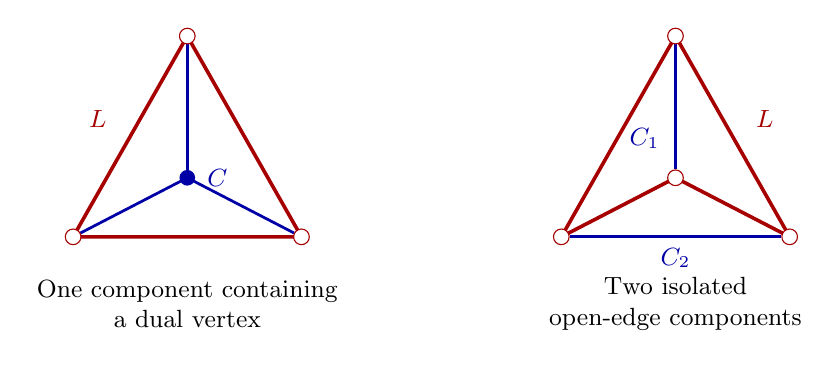
\begin{tikzpicture}[
  wall/.style={red!65!black,line width=1.3pt},
  component/.style={blue!65!black,line width=1pt,shorten <=3pt,shorten >=3pt},
  deleted/.style={circle,draw=red!65!black,fill=white,inner sep=2pt},
  retained/.style={circle,fill=blue!65!black,inner sep=2pt},
  every node/.style={font=\small}]
\begin{scope}[xshift=-3.1cm]
  \coordinate (a) at (0,1.55);
  \coordinate (b) at (-1.45,-1);
  \coordinate (c) at (1.45,-1);
  \coordinate (d) at (0,-.25);
  \draw[wall] (a)--(b)--(c)--cycle;
  \draw[component,shorten >=0pt] (a)--(d);
  \draw[component,shorten >=0pt] (b)--(d);
  \draw[component,shorten >=0pt] (c)--(d);
  \foreach \v in {a,b,c} \node[deleted] at (\v) {};
  \node[retained] at (d) {};
  \node[blue!65!black,right] at (.13,-.25) {$C$};
  \node[red!65!black,left] at (-.9,.5) {$L$};
  \node[align=center] at (0,-1.85)
    {One component containing\\a dual vertex};
\end{scope}
\begin{scope}[xshift=3.1cm]
  \coordinate (a) at (0,1.55);
  \coordinate (b) at (-1.45,-1);
  \coordinate (c) at (1.45,-1);
  \coordinate (d) at (0,-.25);
  \draw[wall] (a)--(b)--(d)--(c)--cycle;
  \draw[component] (a)--(d);
  \draw[component] (b)--(c);
  \foreach \v in {a,b,c,d} \node[deleted] at (\v) {};
  \node[blue!65!black,left] at (-.08,.25) {$C_1$};
  \node[blue!65!black,below] at (0,-1.02) {$C_2$};
  \node[red!65!black,right] at (.9,.5) {$L$};
  \node[align=center] at (0,-1.85)
    {Two isolated\\open-edge components};
\end{scope}
\end{tikzpicture}
\end{document}
